\documentclass[a4paper,10pt]{article}
\usepackage[utf8]{inputenc}
\usepackage{graphicx}
\graphicspath{{../img/}}
\usepackage{geometry}
\geometry{margin=2cm}

\title{lib\_aec: Test Cases}
\author{Oscar Bailey}

\begin{document}

\maketitle

\section{Method}

To test the AEC, we must supply two audio inputs: a microphone input (AudioIn)
and a far-end input (AudioRef). The microphone input is a combination of desired
near-end audio and noise from the environment. After processing AudioIn and
AudioRef, the AEC outputs two independent audio tracks: AudioOut, and a copy of
the original AudioRef. AudioOut should be similar to the microphone input minus
the noise produced by the far-end input. The noise produced by the far-end input
will change depending on how the sound is reflected in the environment.

This document outlines test cases when the input for the AEC is simulated.  The
tests use a set of chosen parameters: Near-end Audio, AudioRef, and the transfer
function of the room H(). AudioIn will be generated by summing the near-end
audio with H(AudioRef). The AEC will be executed on AudioIn and AudioRef,
producing AudioOut = AudioIn - $\hat{H}$(AudioRef) where $\hat{H}$() is the
model of H() internal to the AEC. AudioOut will be compared to the near-end
audio, producing a pass/fail result based on similarity within a chosen
threshold.

Using simulated input allows us to focus only on cancelling noise created by
AudioRef. When using real audio, AudioIn = G(x) + H(y) where G is the transfer
function describing the effect of the environment on near-end signal x.
Therefore, a perfect AEC operating on recorded audio will generate AudioOut =
G(x). In comparison, by artificially constructing AudioIn = x + H(y) a perfect
AEC will generate AudioOut = x.

To pass a test, the AEC must produce an AudioOut that is sufficiently similar to
the near-end audio. The method of comparison is illustrated in figure
\ref{fig-similar}. Peaks in the frequency domain of the near-end audio should be
present in AudioOut with a magnitude greater than -5dB relative to the near-end
audio. Frequencies which are not present in the near-end audio should be less
than -30dB in AudioOut relative to the largest magnitude in AudioOut.

For the first 60 seconds of processing, the AEC operates with silent near-end
audio i.e. AudioIn = H(y) and AudioRef = y. This ensures that the AEC has
time to adapt its internal model of the room's transfer function and settle to a
stable internal state.

An alternative test method is used to capture the impulse response of the
transfer function internal to the AEC and compare it to the transfer function of
the room. In this test, the input audio is silent followed by a single negative
impulse. After the negative impulse, the AEC is processed without adaptation
enabled. The resulting AudioOut is compared to the room transfer function.
The test passes if they are similar.

When the transfer function of the room is longer than the length of the transfer
function internal to the AEC, we expect that the AEC will not remove the far-end
signal. In this case, the test fails if AudioOut is similar to the near-end
audio.

We will test the performance of the AEC when using multiple channels on both the
AudioIn and AudioRef inputs. In this case, each microphone has an independent
model of the transfer function of the room. Each channel of the reference audio
will have a different reverberation path from the speaker to the mic input.
Therefore, for an M channel reference and an N channel microphone we will
require M$\cdot$N transfer functions to model the room.

As previously mentioned, the AEC outputs both AudioOut and a copy of AudioRef.
We will compare the AudioRef output with the AudioRef input to test whether the
AEC is distorting AudioRef while processing the input audio.

\section{Construction}

The transfer function of the room is visualised in figure \ref{h-plots}. Table
\ref{tab-tests} describes test instances.

\subsection{Reference Signal}

These tests will use reference signals with varying spectral power
distributions, and difference levels of auto-correlation. In preliminary tests,
white noise as a reference signal has performed well.  White noise has a wide,
uniform spectral power distribution and no autocorrelation.

We will also use reference signals which oscillate between a minimum and maximum
frequency. The period of the oscillation will be greater than the excessive echo
transfer functions, and therefore longer than the length of $\hat{H}()$. The
two types of oscillation, discrete and continuous, are visualised in figure
\ref{fig-ref}. The discrete 2-tone oscillating signal has some auto correlation
and a small spectral power distribution. The continuous 2-tone signal has low
auto correlation and a wide spectral power distribution.

To create a reference signal with a small spectral power distribution and high
autocorrelation we will use a sine wave of constant frequency.

The reference signal output by the AEC will be compared sample-by-sample with
the input reference signal. If they are not identical, the test will fail. This
check will be performed for all tests.

\subsection{Near-end Signal}

The frequencies used for near-end audio will be within the range of human
speech.

\subsection{Headroom}

To test for clipping and overflow errors during processing, the audio will be
shifted right 2, 4, and 8 bits. The audio is stored as a sequence of 16 bit
integers, so a right-shift by 8 bits removes half the precision. The spec
dictates that at least 2 bits of headroom is required.


\begin{table}[h]
    \centering
\begin{tabular}{l|l|l|l|l}
    Test Name & HR Bits & Near-end Audio  & Room & AudioRef \\
    \hline
 Simple Tests
 & \{2,4,8\} & Single frequency           & \{Small Echo,      & \{Discrete, \\
 &           &                            & Long Echo,         & Continuous \\
 &           &                            & Decaying Echo\}    & Single Sine,\\
 &           &                            &                    & White Noise\}\\
 \hline
 Multi-tone Tests
 & \{2,4,8\} & Multiple frequency         & \{Small Echo,      & \{Discrete, \\
 &           &                            & Long Echo,         &  Continuous,\\
 &           &                            & Decaying Echo\}    & Single Sine, \\
 &           &                            &                    & White Noise\}\\
 \hline
 Impulse Response Tests
 & \{2,16\} & Silence + Negative Impulse & \{Small Echo,      & \{Discrete, \\
 &           &                            & Long Echo,         &  Continuous,\\
 &           &                            & Decaying Echo\}    & Single Sine,\\
 &           &                            &                    & White Noise\}\\
 \hline
 Excessive Echo Test
 & 8         & Single frequency           & Excessive Echo     & White Noise \\
 \hline
 Band Limited Test
 & 4         & Multiple frequency         & Random             & Band-limited\\
 & & & & White Noise\\
\end{tabular}
\caption{Table of test instances.}
\label{tab-tests}
\end{table}

\begin{figure}[h]
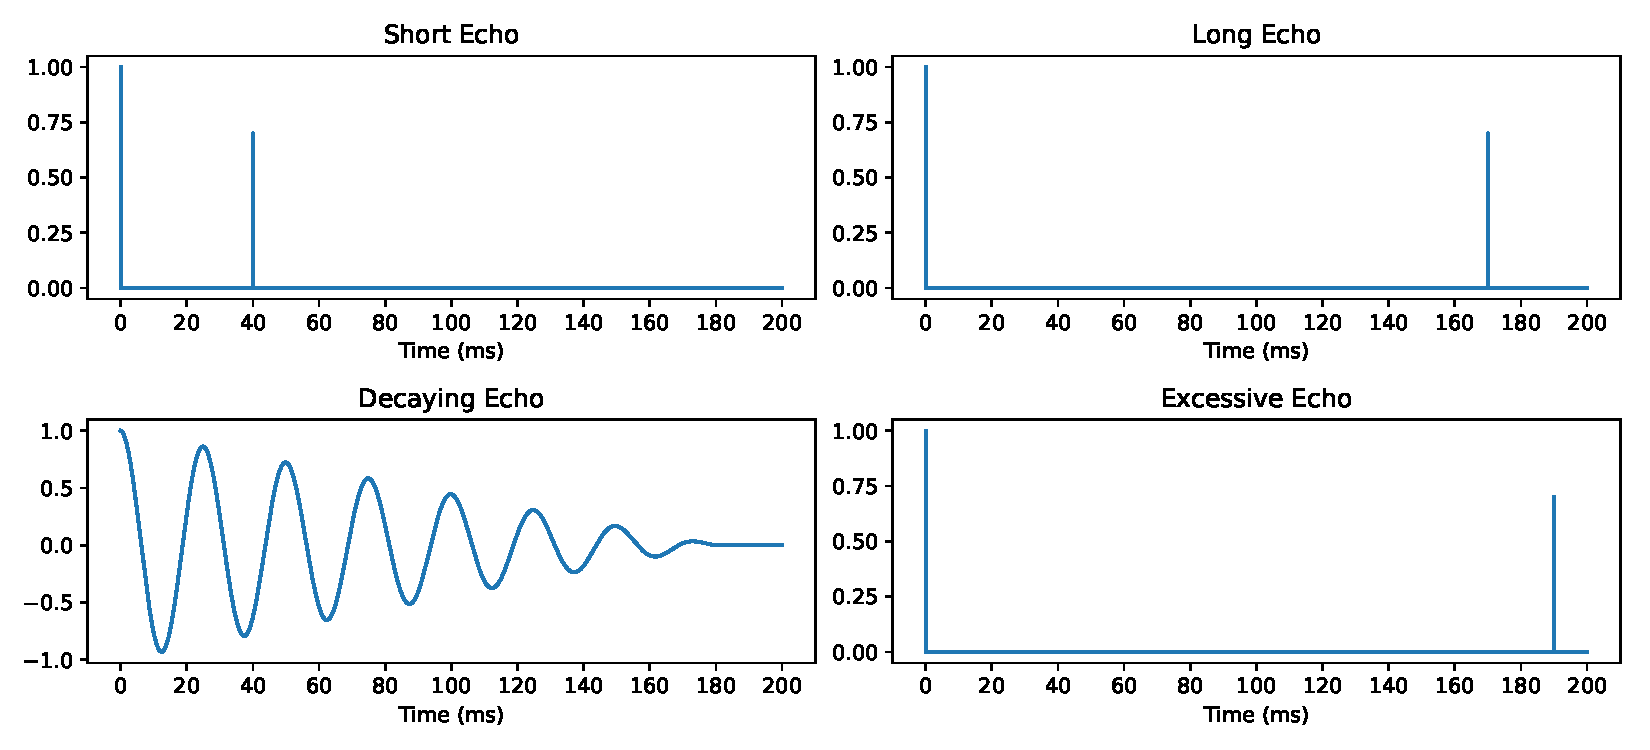
\includegraphics[width=\textwidth]{H}
\caption{Impulse responses of different transfer functions used for testing.}
\label{h-plots}
\end{figure}

\begin{figure}[h]
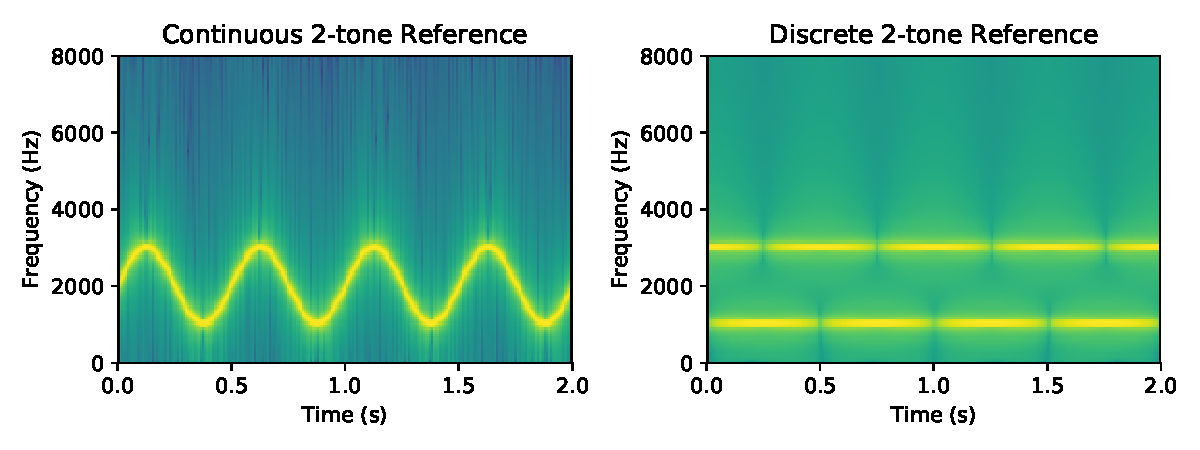
\includegraphics[width=\textwidth]{reference}
\caption{Discrete and Continuous versions of the 2-tone oscillating reference
signal.}
\label{fig-ref}
\end{figure}

\begin{figure}[h]
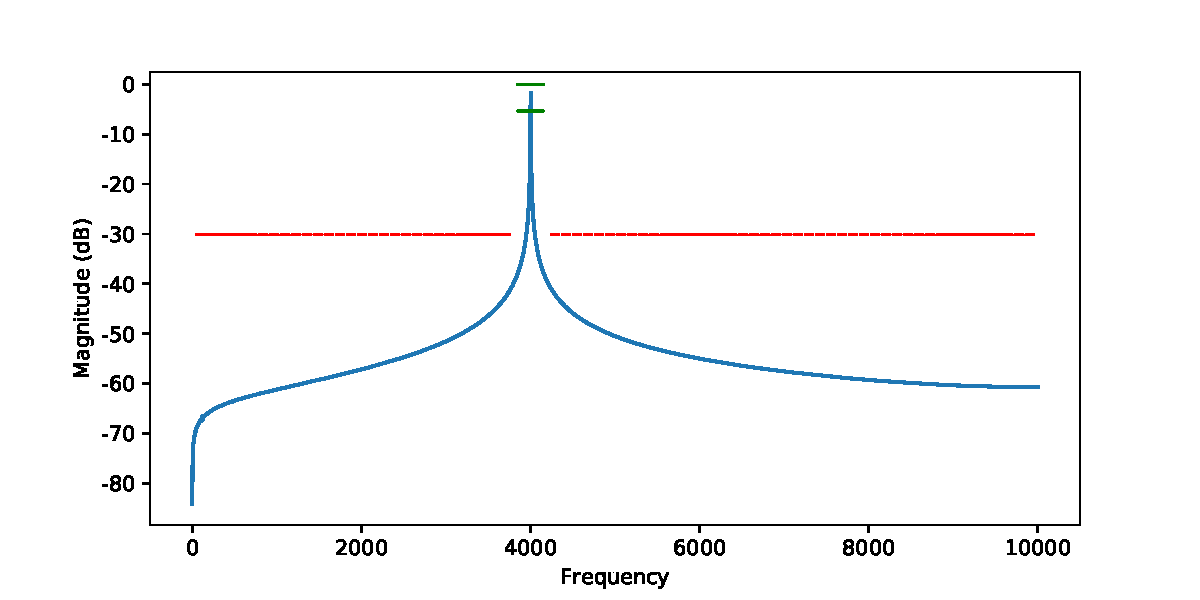
\includegraphics[width=\textwidth]{single-freq}
\caption{Frequency spectrum of single-frequency near-end audio. The red lines
show where the frequency should be below 30dB, and the green lines show the
frequency of greatest magnitude.}
\label{fig-similar}
\end{figure}

\end{document}
